\documentclass{report}
% Change "article" to "report" to get rid of page number on title page
\usepackage{amsmath,amsfonts,amsthm,amssymb}
\usepackage{setspace}
\usepackage{Tabbing}
\usepackage{fancyhdr}
\usepackage{lastpage}
\usepackage{extramarks}
\usepackage{chngpage}
\usepackage{soul,color}
\usepackage{listings}
\usepackage{enumerate}
\usepackage{graphicx,float,wrapfig}
\usepackage{pifont}
\usepackage{graphicx}
\usepackage[english]{babel}
\usepackage{tikz}
% In case you need to adjust margins:
\topmargin=-0.45in      %
\evensidemargin=0in     %
\oddsidemargin=0in      %
\textwidth=6.5in        %
\textheight=9.0in       %
\headsep=0.25in         %

\title{Assignment 4 - Comp 5361 - Discrete Math}

% Homework Specific Information
\newcommand{\hmwkTitle}{Assignment 4}                     % Adjust this
\newcommand{\hmwkDueDate}{Thursday, March 13 2014}                           % Adjust this
\newcommand{\hmwkClass}{COMP 5361}


\newcommand{\hmwkClassInstructor}{Dr. Stan Klasa}
\newcommand{\hmwkAuthorName}{Geoffrey Stanley}
\newcommand{\hmwkAuthorNumber}{5064961}
\newcommand{\Pp}{\mathbb{P}}
\newcommand{\Ev}{\mathbb{E}}
\newcommand{\cov}{\text{Cov}}
\newcommand{\Z}{\mathbb{Z}}
\newcommand{\R}{\mathbb{R}}
\newcommand{\dd}{\, \mathrm{d}}

% Setup the header and footer
\pagestyle{fancy}                                                       %
\lhead{\hmwkAuthorName}                              %
\chead{}
\rhead{\hmwkClass: \hmwkTitle}                                          %

\lfoot{}
\cfoot{}                                                                %
\rfoot{Page\ \thepage\ of\ \pageref{LastPage}}                          %
\renewcommand\headrulewidth{0.4pt}                                      %
\renewcommand\footrulewidth{0.4pt}                                      %

% This is used to trace down (pin point) problems
% in latexing a document:
%\tracingall
\definecolor{mygreen}{rgb}{0,0.6,0}
\lstset{commentstyle=\color{mygreen}, frame=single,  language=R, showspaces=false, showstringspaces=false}

%%%%%%%%%%%%%%%%%%%%%%%%%%%%%%%%%%%%%%%%%%%%%%%%%%%%%%%%%%%%%
% Make title
\title{\vspace{2in}\textmd{\textbf{\hmwkClass:\ \hmwkTitle}}\\\normalsize\vspace{0.1in}\small{Due\ on\ \hmwkDueDate}\\\vspace{0.1in}\large{\textit{Presented to \hmwkClassInstructor}}\vspace{3in}}
\date{}
\author{\textbf{\hmwkAuthorName}\\
    \textbf{Student ID: \hmwkAuthorNumber}}
%%%%%%%%%%%%%%%%%%%%%%%%%%%%%%%%%%%%%%%%%%%%%%%%%%%%%%%%%%%%%

\begin{document}
\maketitle
I certify that this submission is my original work
and meets the Faculty's
Expectations of Originality.\\
\section*{Question 1}
\subsection*{A)}
$a(bb)^*(ab)^*$\\
Let $L$ represent the regular language described by $a(bb)^*(ab)^*$.\\

Given the definition of $L$ words must start with an $a$ and be followed by $bb$ or $ab$.\\

In order to form the word $abab$ one must be able to follow $a$ with $ba$. As such, it is impossible to construct the word $abab$ with this language $L$.
\subsection*{B)}
$ab^*a^*$\\
Let $L$ represent the regular language described by $ab^*a*$.\\

Given the definition of $L$ words must start with an $ab$ and be followed by $b$ or $a$.\\

In order to form the word $abab$ one must be able to follow $ab$ with $ab$. As such, it is impossible to construct the word $abab$ with this language $L$.
\subsection*{C)}
$a(ba)^*b^*$\\
Let $L$ represent the regular language described by $a(ba)^*b^*$.\\

Given the definition of $L$ one can assign a value of $1$ to the first and second exponent. This would result in $abab$.\\

As such, it is possible to construct the word $abab$ with this language $L$.
\subsection*{D)}
$a^*ba(a\cup b)$\\
Let $L$ represent the regular language described by $a^*ba(a\cup b)$.\\

Given the definition of $L$ one can assign a value of $1$ to the first exponent and choose b over a in $(a\cup b)$. This would result in $abab$.\\

As such, it is possible to construct the word $abab$ with this language $L$.
\subsection*{E)}
$(ab)^*(bb)^*$\\
Let $L$ represent the regular language described by $(ab)^*(bb)^*$.\\

Given the definition of $L$ one can assigns a value of $2$ to the first exponent and $0$ to the second exponent. This would result in $abab$.\\

As such, it is possible to construct the word $abab$ with this language $L$.
\subsection*{F)}
$a^*(ba \cup bb)^*$\\
Let $L$ represent the regular language described by $a^*(ba \cup bb)^*$ and $wL$ be a word formed with this language.\\

Given the definition of $L$ words must start with a $a$, $ba$ or $bb$. The only scenario where it would be possible to form the words $abab$ is if $wL$ begins with $a$. Following $a$ the only options are $ba$ or $bb$ followed again by $ba$ or $bb$.\\

In order to form the word $abab$ one must be able to follow $a$ with $bab$. As such, it is impossible to construct the word $abab$ with this language $L$.
\subsection*{G)}
$a^*(ba)^*bb$\\
Let $L$ represent the regular language described by $a^*(ba)^*bb$ and $wL$ be a word formed with this language.\\

Given the definition of $L$ words must start with a $a$, $ba$ or $bb$. The only scenario where it would be possible to form the words $abab$ is if $wL$ begins with $a$. Following $a$ the only options are $ba^*$ or $bb^*$.\\

In order to form the word $abab$ one must be able to follow $a$ with $bab$. As such, it is impossible to construct the word $abab$ with this language $L$.
\subsection*{H)}
$ab(ab \cup a)b^*$\\
Let $L$ represent the regular language described by $ab(ab \cup a)b^*$.\\

Given the definition of $L$ one can assigns a value of $0$ to the exponent and choose ab over a. This would result in $abab$.\\

As such, it is possible to construct the word $abab$ with this language $L$.
\section*{Question 2}
\subsection*{A)}
\begin{center}
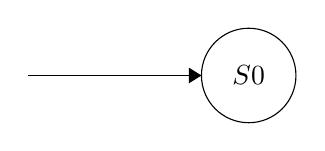
\begin{tikzpicture}[scale=0.2]
\tikzstyle{every node}+=[inner sep=0pt]
\draw [black] (42.2,-26.9) circle (3);
\draw (42.2,-26.9) node {$S0$};
\draw [black] (28.2,-26.9) -- (39.2,-26.9);
\fill [black] (39.2,-26.9) -- (38.4,-26.4) -- (38.4,-27.4);
\end{tikzpicture}
\end{center}
\subsection*{B)}
\begin{center}
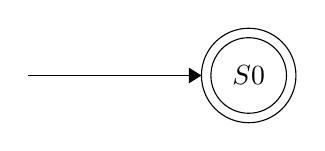
\begin{tikzpicture}[scale=0.2]
\tikzstyle{every node}+=[inner sep=0pt]
\draw [black] (42.2,-26.9) circle (3);
\draw [black] (42.2,-26.9) circle (2.4);
\draw (42.2,-26.9) node {$S0$};
\draw [black] (28.2,-26.9) -- (39.2,-26.9);
\fill [black] (39.2,-26.9) -- (38.4,-26.4) -- (38.4,-27.4);
\end{tikzpicture}
\end{center}
\subsection*{C)}
\begin{center}
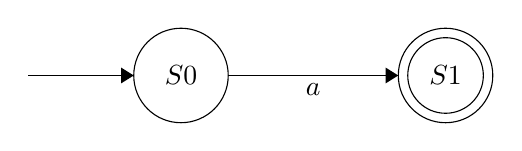
\begin{tikzpicture}[scale=0.2]
\tikzstyle{every node}+=[inner sep=0pt]
\draw [black] (39.9,-27.1) circle (3);
\draw (39.9,-27.1) node {$S1$};
\draw [black] (39.9,-27.1) circle (2.4);
\draw [black] (23.1,-27.1) circle (3);
\draw (23.1,-27.1) node {$S0$};
\draw [black] (13.4,-27.1) -- (20.1,-27.1);
\fill [black] (20.1,-27.1) -- (19.3,-26.6) -- (19.3,-27.6);
\draw [black] (26.1,-27.1) -- (36.9,-27.1);
\fill [black] (36.9,-27.1) -- (36.1,-26.6) -- (36.1,-27.6);
\draw (31.5,-27.6) node [below] {$a$};
\end{tikzpicture}
\end{center}
\section*{Question 3}
\subsection*{A)}
\begin{center}
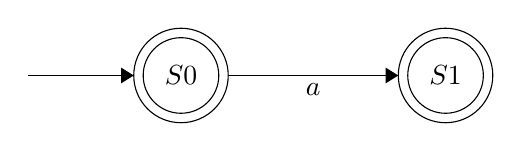
\begin{tikzpicture}[scale=0.2]
\tikzstyle{every node}+=[inner sep=0pt]
\draw [black] (39.9,-27.1) circle (2.4);
\draw [black] (39.9,-27.1) circle (3);
\draw (39.9,-27.1) node {$S1$};
\draw [black] (23.1,-27.1) circle (2.4);
\draw [black] (23.1,-27.1) circle (3);
\draw (23.1,-27.1) node {$S0$};
\draw [black] (13.4,-27.1) -- (20.1,-27.1);
\fill [black] (20.1,-27.1) -- (19.3,-26.6) -- (19.3,-27.6);
\draw [black] (26.1,-27.1) -- (36.9,-27.1);
\fill [black] (36.9,-27.1) -- (36.1,-26.6) -- (36.1,-27.6);
\draw (31.5,-27.6) node [below] {$a$};
\end{tikzpicture}
\end{center}
\subsection*{B)}
\begin{center}
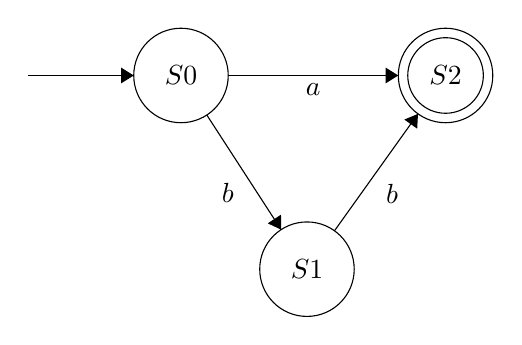
\begin{tikzpicture}[scale=0.2]
\tikzstyle{every node}+=[inner sep=0pt]
\draw [black] (39.9,-27.1) circle (3);
\draw (39.9,-27.1) node {$S2$};
\draw [black] (39.9,-27.1) circle (2.4);
\draw [black] (23.1,-27.1) circle (3);
\draw (23.1,-27.1) node {$S0$};
\draw [black] (31.1,-39.4) circle (3);
\draw (31.1,-39.4) node {$S1$};
\draw [black] (13.4,-27.1) -- (20.1,-27.1);
\fill [black] (20.1,-27.1) -- (19.3,-26.6) -- (19.3,-27.6);
\draw [black] (26.1,-27.1) -- (36.9,-27.1);
\fill [black] (36.9,-27.1) -- (36.1,-26.6) -- (36.1,-27.6);
\draw (31.5,-27.6) node [below] {$a$};
\draw [black] (24.74,-29.61) -- (29.46,-36.89);
\fill [black] (29.46,-36.89) -- (29.45,-35.94) -- (28.61,-36.49);
\draw (26.48,-34.57) node [left] {$b$};
\draw [black] (32.85,-36.96) -- (38.15,-29.54);
\fill [black] (38.15,-29.54) -- (37.28,-29.9) -- (38.1,-30.48);
\draw (36.09,-34.62) node [right] {$b$};
\end{tikzpicture}
\end{center}
\subsection*{C)}
\begin{center}
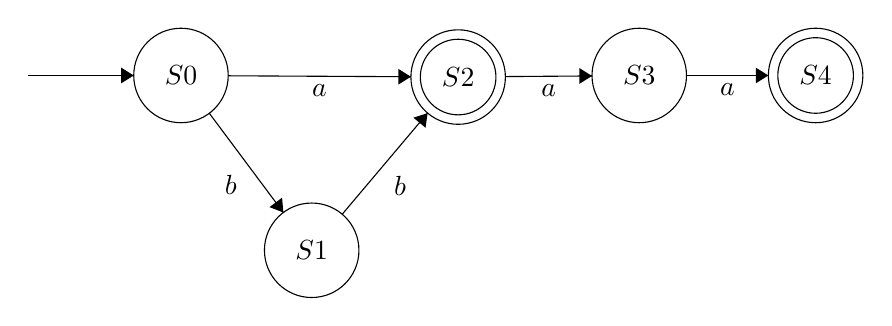
\begin{tikzpicture}[scale=0.2]
\tikzstyle{every node}+=[inner sep=0pt]
\draw [black] (39.9,-27.1) circle (3);
\draw (39.9,-27.1) node {$S2$};
\draw [black] (39.9,-27.1) circle (2.4);
\draw [black] (22.3,-27) circle (3);
\draw (22.3,-27) node {$S0$};
\draw [black] (30.6,-38.1) circle (3);
\draw (30.6,-38.1) node {$S1$};
\draw [black] (51.4,-27) circle (3);
\draw (51.4,-27) node {$S3$};
\draw [black] (62.6,-27) circle (3);
\draw (62.6,-27) node {$S4$};
\draw [black] (62.6,-27) circle (2.4);
\draw [black] (12.6,-27) -- (19.3,-27);
\fill [black] (19.3,-27) -- (18.5,-26.5) -- (18.5,-27.5);
\draw [black] (25.3,-27.02) -- (36.9,-27.08);
\fill [black] (36.9,-27.08) -- (36.1,-26.58) -- (36.1,-27.58);
\draw (31.1,-27.56) node [below] {$a$};
\draw [black] (42.9,-27.07) -- (48.4,-27.03);
\fill [black] (48.4,-27.03) -- (47.6,-26.53) -- (47.6,-27.53);
\draw (45.65,-27.56) node [below] {$a$};
\draw [black] (54.4,-27) -- (59.6,-27);
\fill [black] (59.6,-27) -- (58.8,-26.5) -- (58.8,-27.5);
\draw (57,-27.5) node [below] {$a$};
\draw [black] (24.1,-29.4) -- (28.8,-35.7);
\fill [black] (28.8,-35.7) -- (28.72,-34.76) -- (27.92,-35.36);
\draw (25.87,-33.95) node [left] {$b$};
\draw [black] (32.54,-35.81) -- (37.96,-29.39);
\fill [black] (37.96,-29.39) -- (37.06,-29.68) -- (37.83,-30.32);
\draw (35.8,-34.04) node [right] {$b$};
\end{tikzpicture}
\end{center}
\end{document}
